\documentclass{article}
\usepackage{import}
\subimport{../}{preamble}
\begin{document}

\section{Supplementary Optical Information}

Features, design justifications and optics theory not essential to the main text are detailed here. The following paragraphs clarify the advantages of the reimaging technique, the limitations in choice of objective lens, beamsplitters and optical bench layout. Lastly, further useful information and optics characterisation, such as the range of laser powers, are presented.

\subsection{Optical Design}

\begin{figure}[h]
\centering
\subimport{../3_test_rig_design/figures/}{reimaging_concept.pdf_tex}
\caption*
%[Concept of reimaging for beam alignment]
{\textbf{Concept of reimaging for beam alignment.} Adjusting the angle of the beam in a focal plane does not change the position of the focus in the image (front focal) plane but changes the position in the Fourier (back focal) plane. Adjusting the angle of the beam in a Fourier plane translates the position of the beam in the image plane without changing its angular components.}
\label{fig:reimaging_concept}
\end{figure}

The concept of reimaging, and its effect on beam alignment, is shown in \figurename~\ref{fig:reimaging_concept}. The ray diagrams show that the beam position in the focus can be adjusted by changing the angle of a mirror placed in the Fourier plane (in the case of the microscope the mirror directly after the DF stop). The shape of the beam, dictated by its angular distribution in Fourier space, is controlled by tilting a mirror in a focal plane (the mirror in the focus of the reimaging arm). The two mirrors provide independent control over the two main beam properties.

\begin{figure}[h]
\centering
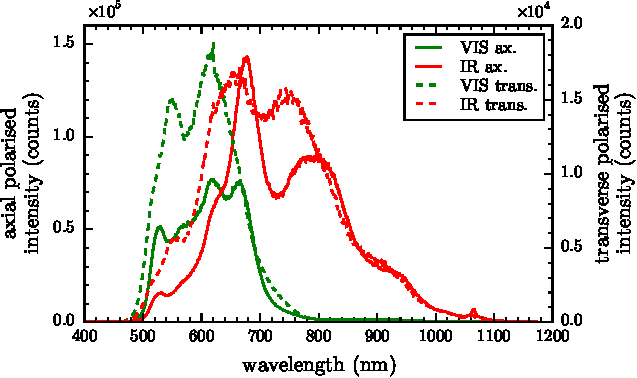
\includegraphics{figures/objective_comparison}
\caption*
%[Spectral comparison between VIS and IR objectives]
{\textbf{Spectral comparison between VIS and IR objectives.} The VIS objective is an Olympus $100\times$ 0.9\,NA MPlan BD dark-field objective whereas the IR objective is an Olympus $100\times$ 0.8\,NA MPlan bright-field objective.}
\label{fig:objective_comparison}
\end{figure}

The choice of objective was determined by the overall range over which a reference spectrum from a Ag mirror is valid. Two long working distance objectives suitable for single nanostructure spectroscopy were characterised for use in the microscope: a VIS and a IR objective. The raw spectra measured using each of the objectives is shown in \figurename~\ref{fig:objective_comparison}. The sharp cut-on at \SI{480}{nm} is due to the supercontinuum laser. The VIS objective clearly outperforms the IR objective below \SI{625}{nm}, though both objective counts are large enough to maintain a good reference signal. Overall, references using the VIS objective only extend marginally more below \SI{500}{nm}. However, the sharp \SI{700}{nm} cut-off in the VIS objective means that it is not suitable for spectra in the NIR. The reference signal of the VIS objective is only valid up until \SI{900}{nm} whereas the IR objective extends to \SI{1100}{nm}. The gain in spectral range means that the IR objective is chosen despite its lack of dark-field illumination for imaging.

\begin{figure}[h]
\centering
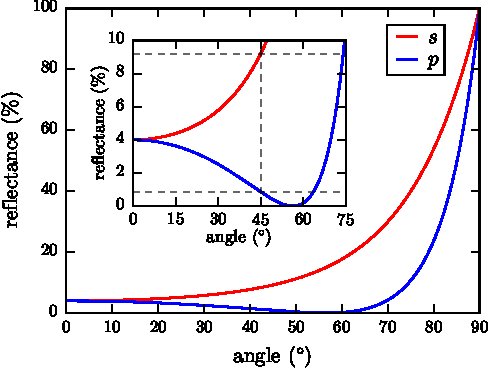
\includegraphics{figures/fresnel_coefficients}
\caption*
%[Reflectance as a function of angle of incidence for glass-air interface]
{\textbf{Reflectance as a function of angle of incidence for glass-air interface.} Reflective is calculated from the fresnel coefficients. The refractive index of glass is assumed to be $n=1.5$. The inset shows a zoomed segment in the low reflectance regime.}
\label{fig:fresnel}
\end{figure}

Consideration was given when designing the optical layout to account for intensity differences in each linear polarisation. Reflection and transmission of an incident EM wave at an interface between two refractive media is characterised by the Fresnel equations, with reflectance given by,
\begin{align}
R_s &= \left| \frac{n_1\cos{\theta_i} - n_2\cos{\theta_t}}{n_1\cos{\theta_i} + n_2\cos{\theta_t}} \right|^2, \\
R_p &= \left| \frac{n_1\cos{\theta_t} - n_2\cos{\theta_i}}{n_1\cos{\theta_t} + n_2\cos{\theta_i}} \right|^2,
\end{align}
where the wave impinges on the interface at an angle $\theta_i$ and refracts into a transmitted angle $\theta_t$ due to the refractive index change from $n_1$ to $n_2$. The angles are related using $n_2\sin{\theta_t} = n_1\sin{\theta_i}$. As shown in \figurename~\ref{fig:fresnel}, there is a large difference in reflectance between linear polarisations at higher angles of indencence. The microscope is designed such that the $s$-polarisation corresponds to light polarised along the tip axis, maximising its transmission to the spectrometers.

\begin{figure}[h]
\centering
\includegraphics{figures/glass_comparison}
\caption*
%[Comparison of NBK7 and UVFS glass refractive index and reflectance]
{\textbf{Comparison of NBK7 and UVFS glass refractive index and reflectance.} Reflectance is calculated at \SI{45}{\degree} where most beamsplitters operate.}
\label{fig:glass_comparison}
\end{figure}

The refractive index of NBK7 and UVFS is calculated using,
\begin{align}
n_{\mathrm{UVFS}} &= \sqrt{1 + \frac{0.6961663\lambda^2}{\lambda^2-0.0684043^2} + \frac{0.4079426\lambda^2}{\lambda^2-0.1162414^2} + \frac{0.8974794\lambda^2}{\lambda^2-9.896161^2}}, \\
n_{\mathrm{NBK7}} &= \sqrt{1 + \frac{1.03961212\lambda^2}{\lambda^2-0.00600069867} + \frac{0.231792344\lambda^2}{\lambda^2-0.0200179144} + \frac{1.01046945\lambda^2}{\lambda^2-103.560653}},
\end{align}

\subsection{Confocal Microscopy}

Mathematically this corresponds to an effective decrease in the width of the \gls{psf}, the intensity distribution of a diffraction-limited point scatterer.
When describing the behaviour of \glspl{psf}, the optical coordinates (\gls{uo},\gls{vo}) are often used instead of $(x,y,z)$ to simplify calculations, where,
\begin{subequations}
\begin{align}
u &= \wvz z\sin^2\alpha, \\
v &= \wvz \sqrt{x^2+y^2}\sin\alpha,
\end{align}
\end{subequations}
with $\alpha$ as the half angle of light from the aperture. The intensity of an image formed coherently in a confocal microscope is given by $I=|(h_1h_2) \ast \tau|^2$, where $h_1$ and $h_2$ are the \glspl{psf} of illumination and collection apertures and $\tau$ is the optical response of the object. In this case $\tau(0,v)=\delta(v)$ is a point scatterer therefore $I=|h_1h_2|^2$. Convolution of the illumination and confocal \glspl{psf} leads to an image \gls{psf} given by $I_{\mathrm{confocal}} = \left({2J(v)}/{v}\right)^4$ as opposed to the wide-field image PSF of $I_{\mathrm{wide-field}} = \left({2J(v)}/{v}\right)^2$. The FWHM, and therefore the minimum resolvable size, decreases by $\sqrt{2}$ in the confocal case.

A decrease in the Rayleigh criterion \cite{born1999principles} for diffraction-limited resolution, \gls{r_lat}, given by,
\begin{equation}
	r_{\mathrm{lateral}}=\frac{1.22\lambda}{(\NA_{\mathrm{obj}}+\NA_{\mathrm{cond}})}=\frac{0.61\lambda}{\NA},
\end{equation}
in expected in an epi-illumination geometry, to around \cite{},
\begin{equation}
	r_{\mathrm{lateral}}=\frac{0.37\lambda}{\NA}.
\end{equation}
The axial resolution, \gls{r_ax}, is also improved to,
\begin{equation}
	r_{\mathrm{axial}} = \sqrt{\left(\frac{n\lambda}{\NA^2}\right)^2 + \left(\frac{\sqrt{2}nd_{p}}{\NA}\right)^2}.
\end{equation}
Decreasing the pinhole diameter not only decreases the thickness of the optical section but the minimum resolvable lateral distance.

Realistically, however the detector is not a point detector but a finite aperture, so the collection \gls{psf} must be convoluted with the detector rect function, $D$, giving an image \gls{psf} $I=|h_1|^2(|h_2|^2\ast D)$. The FWHM of the image intensity retains the $\sqrt{2}$ improvement if the detector width $v_p\leq0.5$, but realistically this leads to a significant loss in brightness. Resolution is improved until $v_p\geq4$, at which point the wide-field behaviour is recovered. Practically $v_p\leq2$ to optimise lateral resolution and $v_p\leq4$ to optimise depth resolution. The optimum pinhole diameter is calculated using,
\begin{equation} \frac{M}{\mathit{NA}}\geq\frac{\pi d_p}{v_p\lambda}, \end{equation}
where \gls{pinhole} is the pinhole diameter. A sufficiently small pinhole diameter will have $v_p=2$, therefore for a 0.8\,NA, $M=56$ system $d_p/\lambda\leq45$, e.g. \SI{22}{\micro\metre} at \SI{500}{nm} and \SI{50}{\micro\metre} at \SI{1100}{nm}.

\subsection{Characterisation}

\begin{figure}[h]
\centering
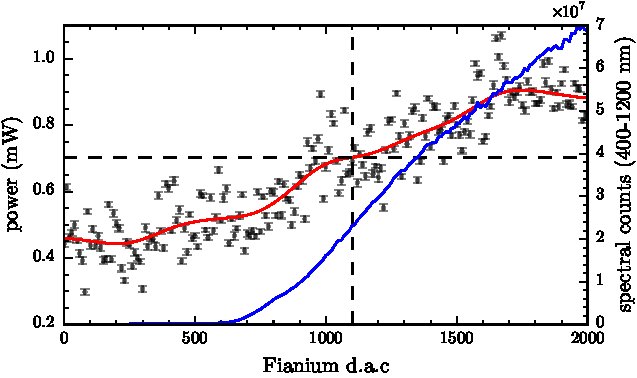
\includegraphics{figures/fianium_power}
\caption*
%[Fianium power incident on the back aperture of the objective as a function of driving current.]
{\textbf{Fianium power incident on the back aperture of the objective as a function of driving current.} The beam diameter is restricted to the size of the back aperture to accurately measure the power throughput without measuring extra power not transmitted to the sample plane. Error bars represent the precision (standard error) of 1000 repeat measurements at each power, hence they are small, however the large distribution of points shows that the power meter is only accurate to \SI{1}{mW}.}
\label{fig:fianium_power}
\end{figure}

The measured broadband power incident on the back aperture of the objective (removing the contribution from over-filling of the back aperture using an iris) is shown in \figurename~\ref{fig:fianium_power}. The power is measured using a thermopile bolometer (Coherent Powermax) with simultaneous measurements of the spectral counts of the $s$-polarised signal component summed between 400--\SI{1200}{nm}. The supercontinuum laser is driven with a d.a.c. of 1100 in most experiments. Under these conditions, less than \SI{1}{mW} is used to illuminate samples, enough that reflection from a reference substrate just under saturates the spectrometer counts. Assuming a spot size on \orderof{\SI{1}{\micro\metre}} means a focal intensity of \SI{e8}{\milli\watt\per\centi\metre\squared}. Sub-mW powers are sufficient to maintain good signals without risking damage to nanoscale samples.

% Fast spectroscopy
%The signal passed to the fast spectroscopy path is used to measure spectra on \si{\micro\second} time scales. Light passing through this path is linearly polarised along a pre-determined axis and focussed onto a shutter constructed from a disassembled hard drive. The hard drive is trigged electronically using a TTL pulse from the oscilloscope to synchronise spectra with an electrical signal. Upon triggering the shutter light transmits through to a monochromater with CCD (Horiba Triax 320 with Princeton Instrument Pixis 256E CCD). The trigger pulse also begins a kinetics acquisition on the CCD in which the pixels are streaked from the active region to the read array before being read out. Light is dispersed and focussed onto the end most row of pixels so that the streaking process builds up a spectral image over time.

%\subsection{Time-Resolved Spectroscopy}

%Time-resolved spectroscopy is achieved using a charge-shuffling CCD. Only the furthermost row of pixels is illuminated with the charge shifted one row at a time every exposure period until the entire CCD has been moved into the readout arrays. The time interval recorded during time-resolved spectroscopy is given by,
%\begin{equation} t_{\mathrm{range}} = 256 (t_{\mathrm{exposure}} + t_{\mathrm{shift}}), \end{equation}
%where $t_{\mathrm{exposure}}$ is the exposure period of each row of pixels and $t_{\mathrm{shift}}$ is the time taken to shift all pixels by one row. The shift rate is set to \SI{9.2}{\micro\second}.
%Continuous cleans are enabled despite the clean cycle affecting the start time of the acquisition. By only cleaning the single illuminated row the cleaning time can be minimised to \SI{10}{\micro\second}.

\section{Supplementary Electronics}

\begin{figure}[bt]
\centering
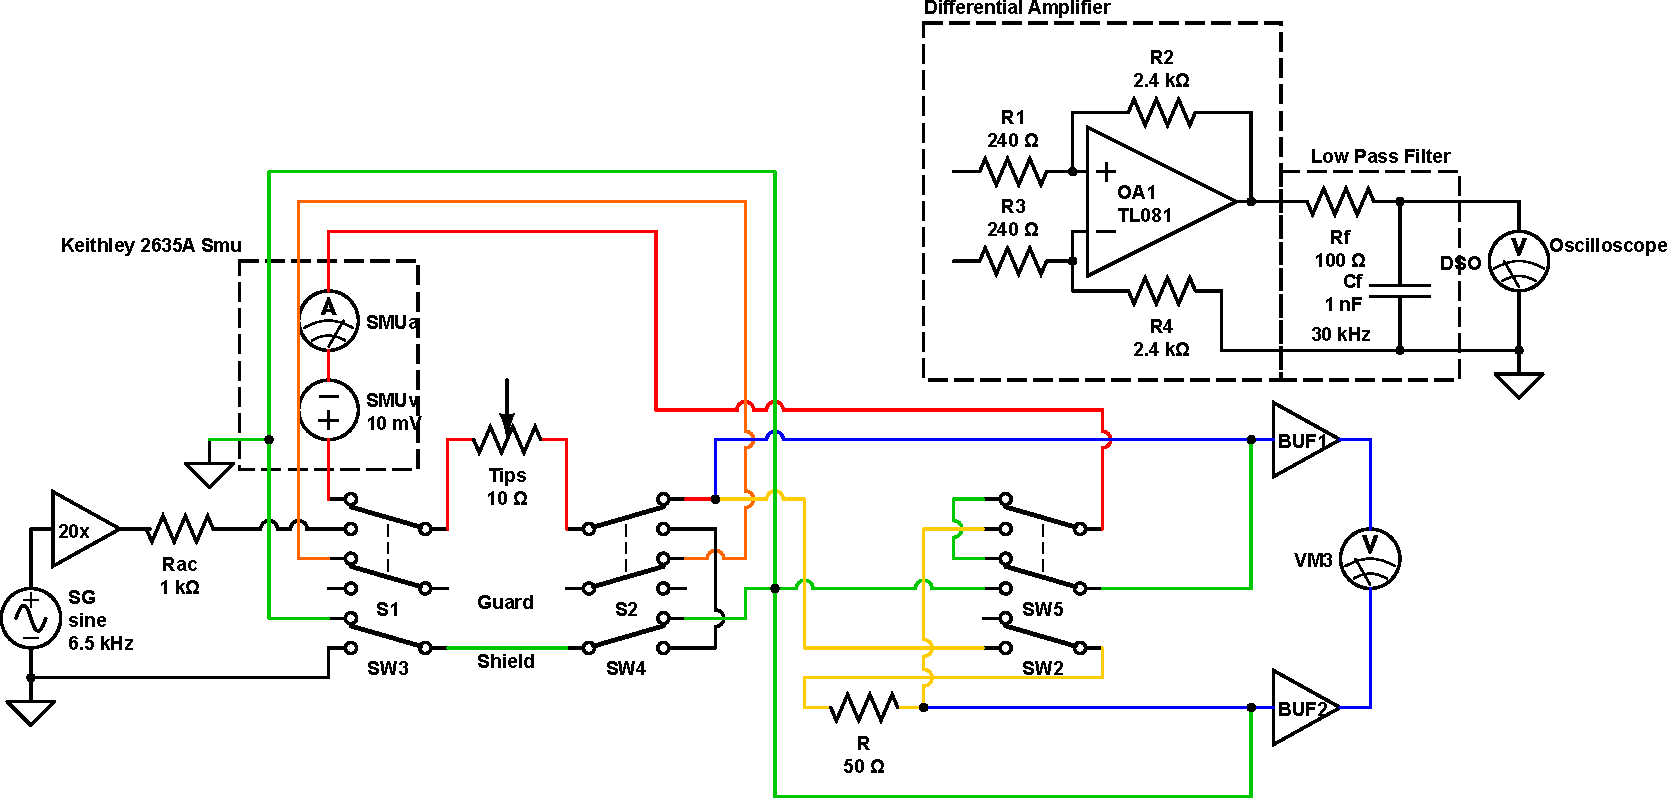
\includegraphics[width=0.9\textwidth]{figures/tip_experiment_circuit_design}
\caption[Schematic of the electrical measurement circuit.]{\textbf{Schematic of the electrical measurement circuit.} The central routing box allows switching between a.c.\ and d.c.\ circuits and low-and high-bandwidth d.c.\ measurements. The a.c.\ circuit is used to align two AFM probes together while the d.c.\ circuit is used to measure spatially dependent signals from the gap between two AFM probes.}
\label{fig:circuit_design}
\end{figure}

The circuitry of the microscope electronics is shown in \figref{fig:circuit_design}

\end{document}